\documentclass[tikz,border=12pt]{standalone}
\usepackage{xcolor}
\begin{document}
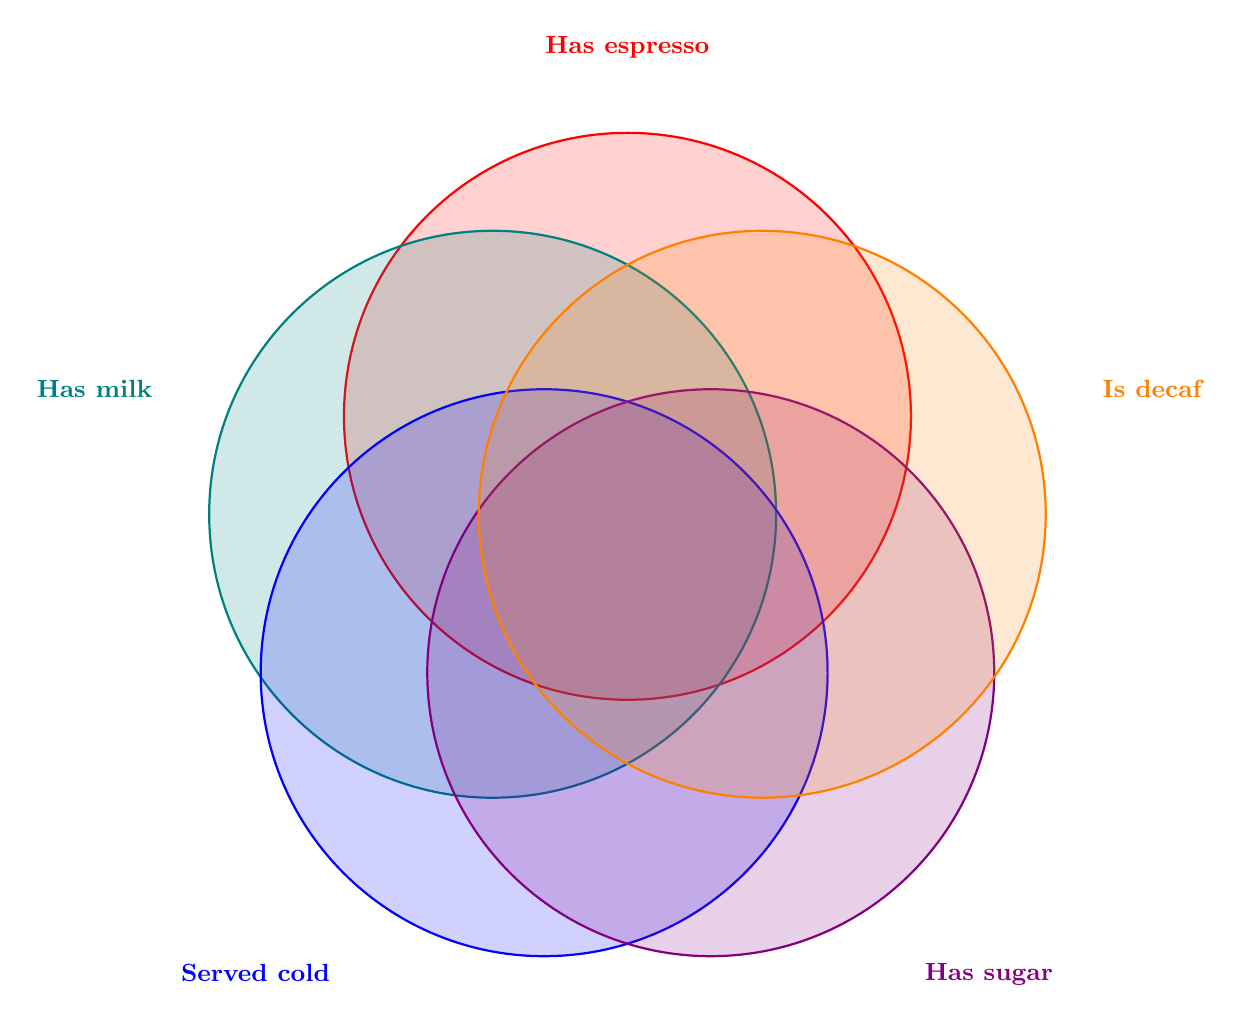
\begin{tikzpicture}[scale=2.4]

% Five circles, centres on a regular pentagon of radius R, each of radius r.
% This arrangement maximises the number of regions obtainable with circles.
\def\R{0.75}
\def\r{1.5}

\foreach \i/\name/\col/\anch in {
  0/Has espresso/red/south,
  1/Has milk/teal/south east,
  2/Served cold/blue/north east,
  3/Has sugar/violet/north west,
  4/Is decaf/orange/south west}
{
  \pgfmathsetmacro{\ang}{90 + 72*\i}
  \pgfmathsetmacro{\cx}{\R*cos(\ang)}
  \pgfmathsetmacro{\cy}{\R*sin(\ang)}
  \pgfmathsetmacro{\lx}{(\R+\r+0.34)*cos(\ang)}
  \pgfmathsetmacro{\ly}{(\R+\r+0.34)*sin(\ang)}
  \fill[\col, fill opacity=0.18] (\cx,\cy) circle (\r);
  \draw[\col, thick] (\cx,\cy) circle (\r);
  \node[\col, anchor=\anch, font=\bfseries\small] at (\lx,\ly) {\name};
}

\end{tikzpicture}
\end{document}
